
\providecommand{\myrootdir}{..}
\documentclass[\myrootdir/main.tex]{subfiles}

\begin{document}

\chapter{LogChunks Data Set}
\label{sec:data-set}
\includegraphics[page=5, width=\textwidth, trim={0.5cm 0.5cm 0.5cm 0.5cm}, clip]{img/flow-of-research.pdf}
This chapter describes the creation of the \emph{LogChunks} data set.
\emph{LogChunks} encompasses about 800 build logs produced by a wide variety of programming languages.
For each build log we manually labeled which substring describes why the build failed.
Four our evaluation of the chunk retrieval techniques PBE, CTS and KWS we added search keywords and structural categories to each of the labeled substrings.

First, we present related data sets and show how \emph{LogChunks} differs.
Second, this chapter describes our log collection process and details the data schema of \emph{LogChunks}.
Further, it presents the labeling process and how we validated the obtained data points.
In our first validation study, a second person also labeled a sample of the build logs.
For the second validation study, we sent out mails to the original project developers to determine whether the substring we labeled actually describes the reason the build failed.

\section{Motivation}
% For our study, described in Chapter~\ref{sec:study}, we want to investigate the retrieval capabilities of three techniques.
% Therefore, we need a data set of in/output examples for one \texttt{BuildLogInformation}.
% Furthermore, Keyword search is not configured by such in/output, but search keywords surrounding the desired output.
% Finally, this section describes our notion of structural categories, which we use to quantify our assumptions on the needed uniformness of in/output examples
In/output examples (I/O examples) are used to configure two of the information retrieval techniques we are evaluating for this thesis, PROSE regular expression program synthesis by example and text similarity.
One example set always contains build log in/output examples from the same software repository or project and for one specific build log information. They are all from one repository because we investigate information retrieval techniques which are always configured to the scope of one particular software repository or project.
Our intuition was that the ability of PROSE to be able to successfully learn a regex program depended on the structural uniformity of the provided in/output examples.
The regular expressions need a consistent pattern in the build log string at the borders or around the textual representation of a build log information to match on for the retrieval.
To be able to quantify this intuition in our evaluation we assigned \emph{structural categories} to each of the examples within an example set.

\section{Related Data Sets}

\paragraph{TravisTorrent}
The \emph{TravisTorrent} data set~\cite{beller2017travistorrent} collects a broad range of metadata about builds on Travis CI.
It combines data accessible through the public Travis CI API~\cite{travisci2019apidoc}, related data from GHTorrent~\cite{gousios2013ghtorrent}, the corresponding git repository and data obtained through analysis of the build logs.
The data obtained through build logs contains the names of failing test cases, similar to the reason the build failed in \emph{LogChunks}.
However, these values are obtained through a manually developed parser, which only supports specific Ruby test runners and Java Maven or JUnit logs.
\emph{LogChunks} provides manually labeled data points on the description of the build failure reason for a much wider selection of programming languages.

\paragraph{Travis CI Build Log Data Set}
Loriot et al.~\cite{loriot2019dataset, loriot2019styler} collected a large amount of Travis CI build logs from 130 github repositories to analyze their use of the Checkstyle plugin.
They selected Maven repsitories that included the Checkstyle plugin and also used Travis CI.
Their data set only provides the plain build logs, whereas \emph{LogChunks} provides manually analyzed build logs from Travis CI.

\section{Log Collection}
In the following we describe how we select the repositories, builds and Logs for \emph{LogChunks}.
To collect the build logs we built the  \texttt{GHTorrentParser},\texttt{LogCollector} and \texttt{TravisRequester} using Ruby.

\paragraph{Repository Sampling}
First, we determine a set of repositories to query logs from.
Our \texttt{GHTorrentParser} queries the \emph{GHTorrent}~\cite{gousios2013ghtorrent} data set for the most popular languages on GitHub~\cite{github2019website}.
It then retrieves the most popular repositories for a given language.
\emph{Popularity} is defined as the number of watches.
The \texttt{TravisRequester}, our tool querying the Travis API~\cite{travisci2019apidoc}, can then check for a given repository whether it uses Travis CI.

For \emph{LogChunks} we queried GHTorrent from 01/04/2018 for the three most popular repositories of each of the 30 most popular languages.

\paragraph{Build Sampling}
The \texttt{LogCollector} uses the \texttt{TravisRequester} to obtain the newest builds for a given repository.
Wwe use a stratified sampling approach: \texttt{TravisRequester} saves the obtained builds in buckets according to their status.
We encountered the following statuses during our data collection:
\begin{multicols}{3}
\begin{itemize}
	\item created
	\item started
	\item cancelled
	\item passed
	\item errored
	\item failed
\end{itemize}
\end{multicols}
The user of \texttt{TravisRequester} configures how many builds should be checked and how many builds per status should be saved.

To sample the builds for \emph{LogChunks} we let \texttt{TravisRequester} check up to a 1000 builds per repository and kept ten for each status.
We discarded all statuses except one, namely ``failed''~\cite{travis2009buildstatus}, to make the most use of Travis' existing categorization of build status.
%Travis assigns the Status ``failed'' when the build faults in the central script phase.
%``Errored'' is assigned when the build faults during the setup or teardown phase.

\paragraph{Log Sampling}
For each build the \texttt{TravisRequester} then selects a log to download.
Travis CI attributes logs to \emph{jobs}.
A single build can consist of multiple jobs, e.g.\ building the same code version and executing tests in various different testing environments.
A failed build can have successful job executions, as just one failed job leads to the whole build being marked as failed.
\texttt{TravisRequester} queries each build for the first job, which has the same state.
For the selected jobs, the tool queries the Travis API V3 over HTTP to obtains the corresponding build log.

We manually inspected the collected build logs and had to discard logs from three repositories.
One had only one failed build, two others had empty build logs on Travis CI.
In total we collected 798 \todo{check} logs from 80 repositories.

\todo{image! like in travistorrent paper, /draft 10 mins/}

% \section{Collection Process}
% For our initial data collection to get an impression of build logs from various projects and languages we used the \texttt{LogCollector} to gather from the 30 most popular languages, up to 3 repositories using Travis CI each and 3 logs per state for each of those repositories.
% For \emph{LogChunks} we again collected from the same selection of repositories though saved only 10 logs of the state \emph{failed} for each repository.
% our impression?
% \todo{image!}

% \section{Build Failure Reason}
% \todo{WHY? one common information developers and researches might want to extract, intentionally not focus on one structurally clearly defined retrieval   cause that would be simple for PROSE retrieval -> better comparability}


\section{Data Schema}
For each repository, \emph{LogChunks} has a list of \emph{examples}.
Each example consists of:
\begin{itemize}
	\item \textbf{Input:} the relative path to the input build log.
	\item \textbf{BuildFailureReason:} the substring of the log describing the reason the build failed.
	\item \textbf{Keywords:} keywords a developer would use to search for the BuildFailureReason.
	\item \textbf{Category:} a categorization of the structural representation of the BuildFailureReason within the build log.
				The category is relative to the other examples for the same repository.
\end{itemize}
Following, this section describes the BuildFailureReason, Keywords and Category in more detail.
.

\paragraph{BuildFailureReason}
The \emph{BuildFailureReason} is the substring of the build logs that describes why the build failed.
This could be the failing test case, the description of a failed linter rule or a compiler error.
The \emph{BuildFailureReason} is one continuous string cut from the build log.
If there are multiple errors leading for the build to fail, the substring contains the first appearing continuous error descriptions.
\emph{Continuous} means that no lines reporting of normal build behavior are interrupting the error descriptions.
Wherever possible, it does \emph{not} include the log statements describing \emph{that} the build failed, but the description of \emph{why} it failed.
For a few logs we were unable to define the section detailing why the build failed, e.g. because this information was logged in another log file.
In these instances the \emph{BuildFailureReason} contains the lines describing that the build failed.

\paragraph{Keywords}
The \emph{Keywords} contain a list of one to three keywords appearing within the \emph{BuildFailureReason} or in the area around it in the build log.
We aim to select keywords a developer would use to search for the \emph{BuildFailureReason} when inspecting the build log.

\paragraph{Category}
For each repository, we assign \emph{structural categories} to the examples.
The structural category compares how the \emph{BuildFailureReasons} are represented within the build logs.
Build tools highlight their error messages with markings, e.g. starting each line with ``\texttt{ERROR}'', surrounding lines filled with special characters or additional empty log lines.
Two examples fall into the same structural categories if they are surrounded by similar markings.
For most cases, two BuildFailureReason examples which fall into one category are outputted either within the same build phase or by the same build tool.
For each repository, the structural categories are represented as integers, starting at 0 and increased with the next appearing category in chronological build order.

\begin{figure}[htbp]
	\centering
	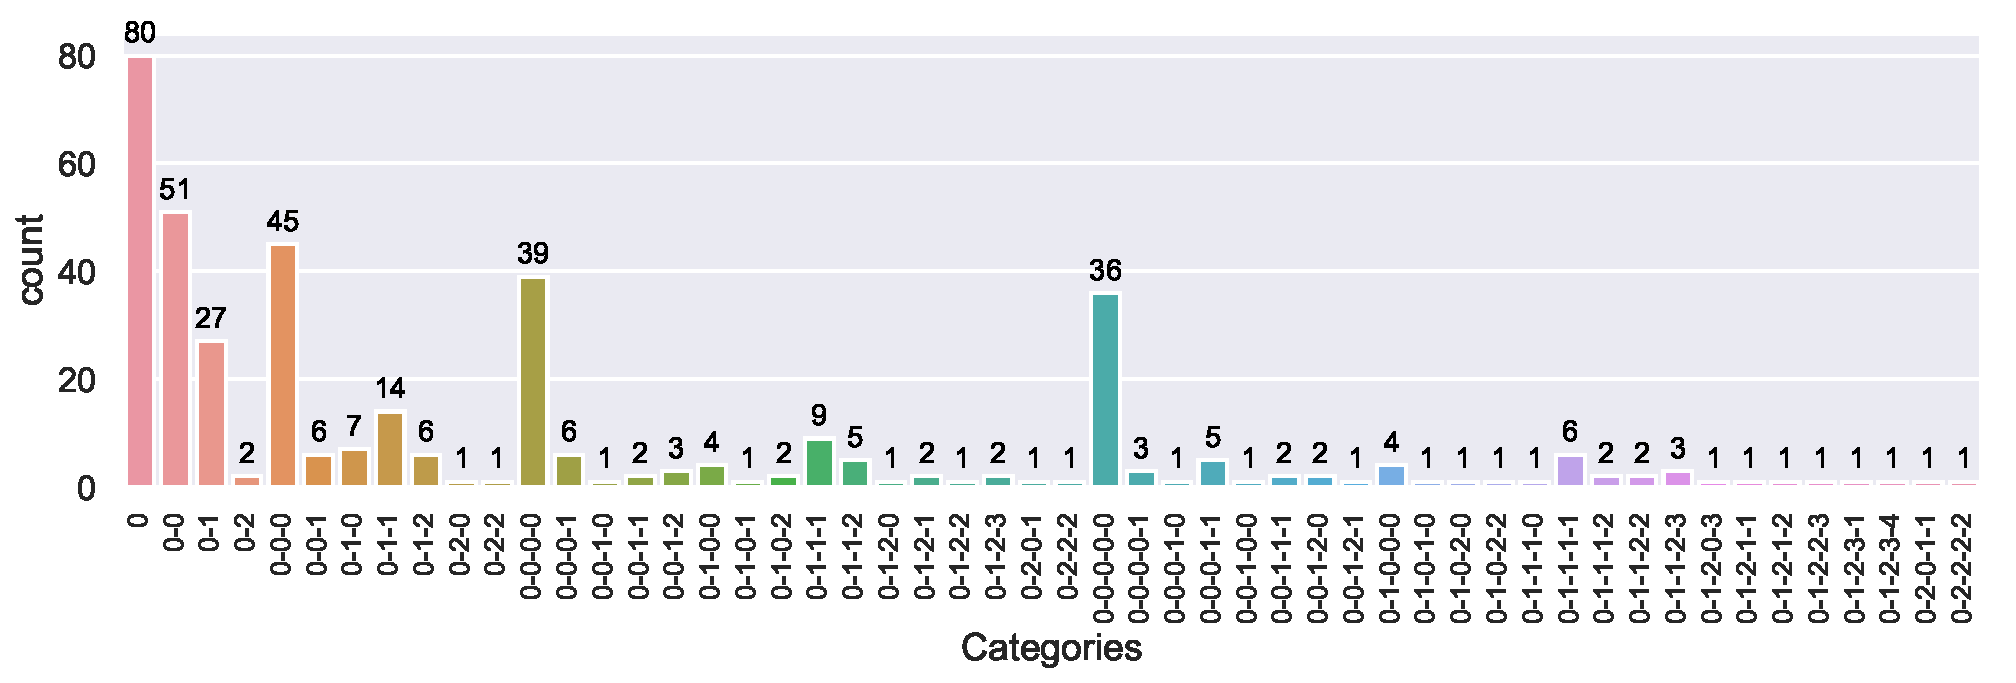
\includegraphics[width=\textwidth, clip]{img/big-study/categories-dataset.pdf}
	\caption{Distribution of the categories in LogChunks}
	\label{fig:categorycount-examplecount-dataset}
\end{figure}

% \paragraph{Example Set}
% \label{sec:example-set}
% Our data set is organized in example sets. One example set always contains build log in/output examples from the same software repository or project and for one specific build log information. They are all from one repository because we investigate information retrieval techniques which are always configured to the scope of one particular software repository or project.
% Each example set has an identifying \emph{save name}, a \emph{build log information} that is desired to be extracted by this configuration, and a list of \emph{in / output examples}.

% \paragraph{In / Output Example}
% In/output examples (I/O examples) are used to configure two of the information retrieval techniques we are evaluating for this thesis, PROSE regular expression program synthesis by example and text similarity.
% In our data set they always consist of an \emph{input path}, linking to the build log file which is the input for this example.
% The \emph{output} is a substring of that build log, the textual representation of the targeted build log information within the input build log.

% \paragraph{Keywords}
% The keyword search is configured by a list of keywords which are searched in the document with plain text search.
% In order to compare it to the two other techniques, each in/output example is associated with a list of 1 - 3 keywords that can be found close to the textual representation of the targeted build log information.

% % \paragraph{Description}
% % \todo{for simple keyword search - imitate what users would search for ad-hoc}

% % \todo{learning steps combining keywords -> similar to how devs would learn from reading those models}

% \paragraph{Categories}
% Our intuition was that the ability of PROSE to be able to successfully learn a regex program depended on the structural uniformity of the provided in/output examples.
% The regular expressions need a consistent pattern in the build log string at the borders or around the textual representation of a build log information to match on for the retrieval.
% To be able to quantify this intuition in our evaluation we assigned \emph{structural categories} to each of the examples within an example set.
% If two retrievals are at the same structural location with the build log, meaning they are surrounded by a similar markings, the fall into the same category.
% For most cases, two build failure reason examples which fall into one category are outputted either within the same build step or by the same build step tool.

\section{Labeling Process}

\paragraph{BuildFailureReason}
For each repository, the labeler skimmed through the build logs and tried to identify the first occurrence of a description why the build failed.
They copied out the first continuous description as the BuildFailureReason.
They preserved whitespace and special characters, as they might be crucial to detect the targeted substring.

\paragraph{Keywords}
We presented the BuildFailureReason substring and ten lines above and below to the labeler.
Their task was to note down three strings they would put into a document search function to find this failure description.
The string should appear in or around the BuildFailureReason substring and is case-sensitive.
There are no special limitations on the string itself, especially spaces are also allowed.
Regular Expressions are not allowed.

\paragraph{Category}
To label the \emph{structural categories} we again presented the BuildFailureReason and the surrounding context to the labeler for all logs from a repository.
We asked them to assign numerical categories according to whether the BuildFailureReason substring had the same structural representation, i.e. the same surrounding or identifying characters.
The labeler should start the categories with 0 and increase as new ones appear.
For reproducibility we presented the logs in chronological build order.


\section{Validation}
We validate our collected data points in two different ways.
A different labeler performed a second pass of labeling the build failure reason, keywords and categories on a subset of the data.
We compared the results to calculate the inter-rater reliability using Cohens kappa.
In addition, we sent out a survey to the developers, whose commits triggered the builds within our data set.
We asked them whether our retrieval of the log part describing the reason the build failed was correct.
This sections describes these two validation studies.

\subsection{Inter-Rater Reliability Study}
re-labeling of parts of the labels - cohen's kappa
\subsubsection{Introduction}
After the manual labeling of the data set we performed a second labeling of a sample of the build logs to validate the labels.
\subsubsection{Method}
For each label category: Build Failure Reason, keywords and category, we relabeled 30 randomly sampled logs.
compared the labels, \todo{discussed about it}.
\subsubsection{Results}

\subsubsection{Discussion}
main takeaway: overlap yes, but high variation 

build failure reason: should we extract the information \emph{that} the build failed as well?
our data set extracts the parts describing \emph{why}, but leaves out the lines stating that the build failed (e.g. step xy exited with 1).

keywords: first labeler allowed also longer strings with spaces and adhered to capitalization.
second one ignored captialization and focussed on the keyword.
so only one word was allowed.
also the first one labeled always a full repository at a time.
so could take into consideration patterns and see what keywords are exception specific and would only retrieve the failure reason if this specific exception occured.
second labeler only one build log excerpt (+ context) per repository.
also: influene of ansi color codes ``merror'' vs. ``error'' first labeler known as ansi color codes, second one counted it into the word (whole word always)
first was also more inclined to search for a subpart of a word to make it more generalizeable (``failure`` instead of ``failures'')

categories: description for the second labeling stated: sort into categories on why build failed.
was exectued with sorting into test/linter/compilation.
in the case of the selected repositories everything was labeled as test. mostly correct (one linter), but more importantly no difference was made in which test step failed / how the failed tests were represented.
the categories are thought as structural categories.
so the surrounding sturcture and the way a test failure is communicated is important. e.g. if several tests are run then it is important which ones failed

main influence / implication: the labels we select are not black/white. accurate description of what we do is very very important. mainly influenced how we described our data points in the earlier sections.
\subsubsection{Threats to Validity}

\subsection{Developer Survey}
\subsubsection{Introduction}
For \emph{LogChunks} we analyzed around 800 build logs from different repositories and tried to extract the part of the log which describes why the respective build failed.
As we are not involved in the development of any of the open source projects within our data set we could only rely on our previous experience with different build logs and systems.
We only looked into the logs and did not check the related configurations, so it is well possible that we extracted parts that do describe errors but the respective step failing is ignored by the configuration and the build failed for another reason.

The person who probably knows best why a build failed is the one committing the changes which triggered the build.
If the build was e.g.\ part of a pull request then developer likely looked at it and tried to fix it so the pull request could be accepted.
In this section we describe how we validate the extractions of the build failure reason \emph{LogChunks} describes.
\subsubsection{Method}
Using the Travis API, for every build log in the data set we looked up the corresponding build and the committer information.
We grouped all commits triggered by one developer and sent out an email to each of them, asking whether the log part selected during our labeling was indeed describing the reason the build failed.Figure~\ref{fig:dev-mail} shows one of the mails sent out.
The email included links to the corresponding commits, build overview and log file.
We asked the receivers to fill out a short survey in case our extraction was not correct.
Look at Figure~\ref{fig:dev-survey} to get an impression of the survey.
In the survey we presented the selected log part and asked the developer to paste in the log part actually describing the failure reason or describe why we were wrong in their own words.
As some of the extractions we labeled are many lines long, we trimmed all down to 10 lines in order to keep the mail readable.

\begin{figure}[h]
	\centering
	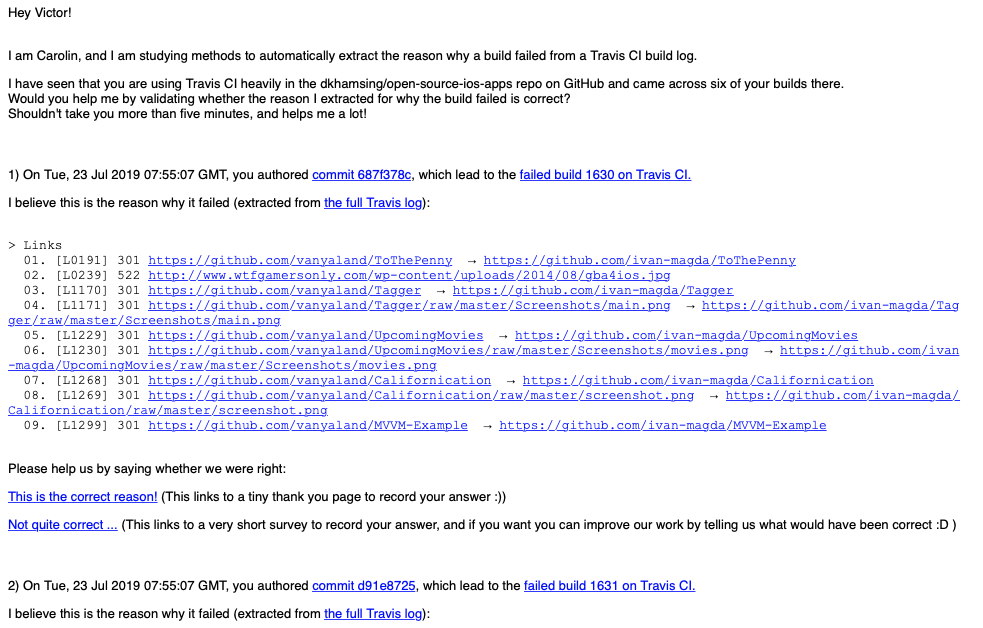
\includegraphics[width=\textwidth, clip]{img/dev-mail.png}
	\caption{An example of the mails we sent out to developers for validation of our labeled log part}
	\label{fig:dev-mail}
\end{figure}
\begin{figure}[h]
	\centering
	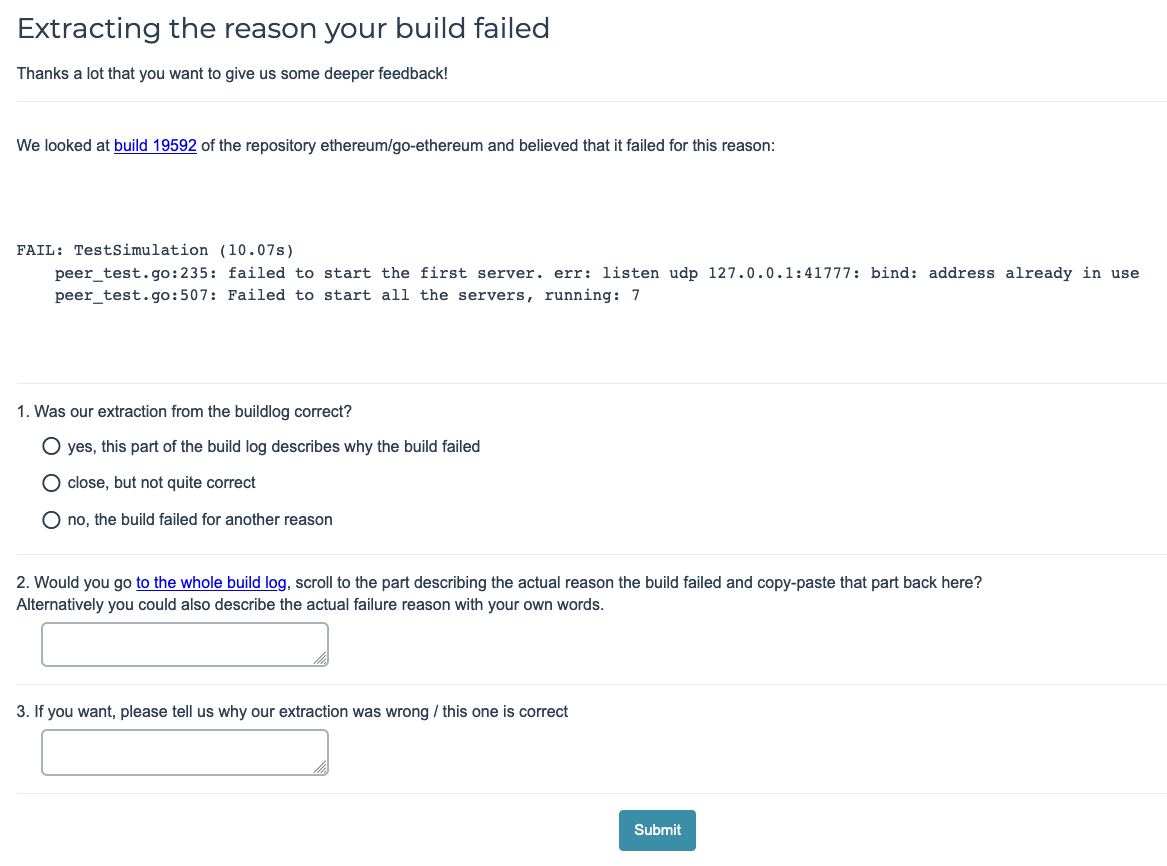
\includegraphics[width=\textwidth, clip]{img/dev-survey.png}
	\caption{Survey for the validation with developers}
	\label{fig:dev-survey}
\end{figure}


\begin{figure}[htbp]
	\centering
	\begin{minipage}{0.45\textwidth}
		\centering
		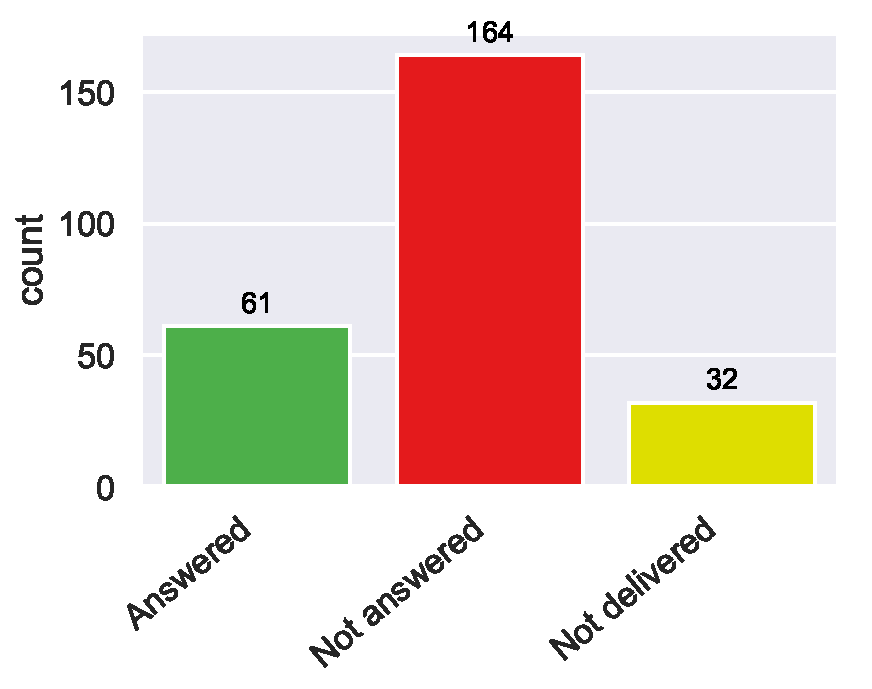
\includegraphics[width=\textwidth, clip]{img/dev-mails/answers-received-mails.pdf}
		\caption{Number of mails answered, unanswered and not delivered}
		\label{fig:mails-answers-received-mails}
	\end{minipage}\hfill
	\begin{minipage}{0.45\textwidth}
		\centering
		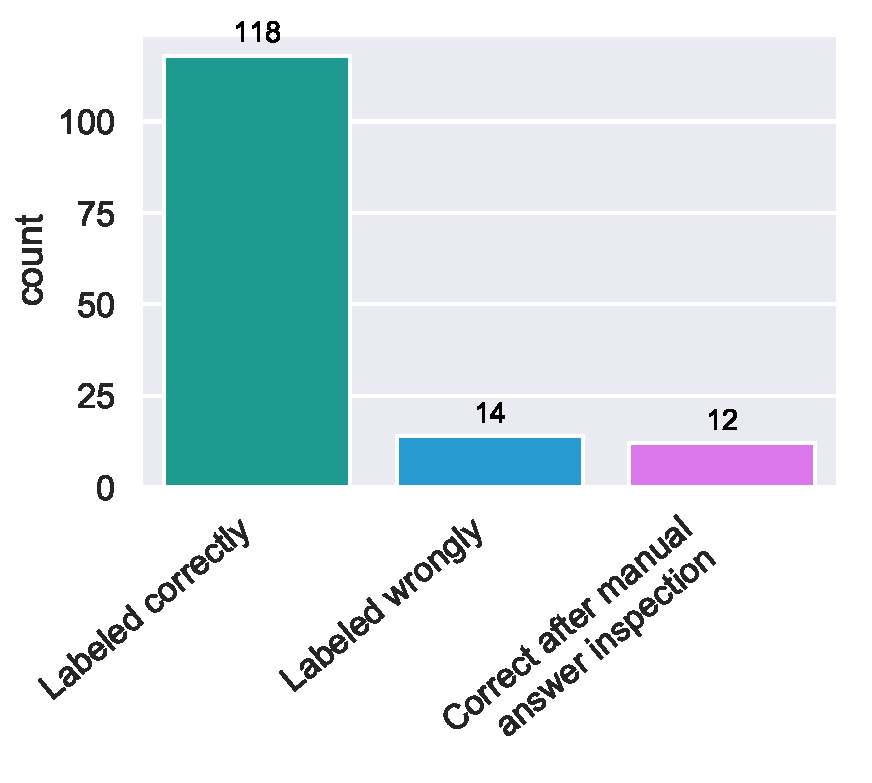
\includegraphics[width=\textwidth, clip]{img/dev-mails/extraction-correct.pdf}
		\caption{Label correctness as validated by developers}
		\label{fig:mails-extraction-correct}
	\end{minipage}
\end{figure}
\begin{figure}[htbp]
	\centering
	\begin{minipage}{0.45\textwidth}
		\centering
		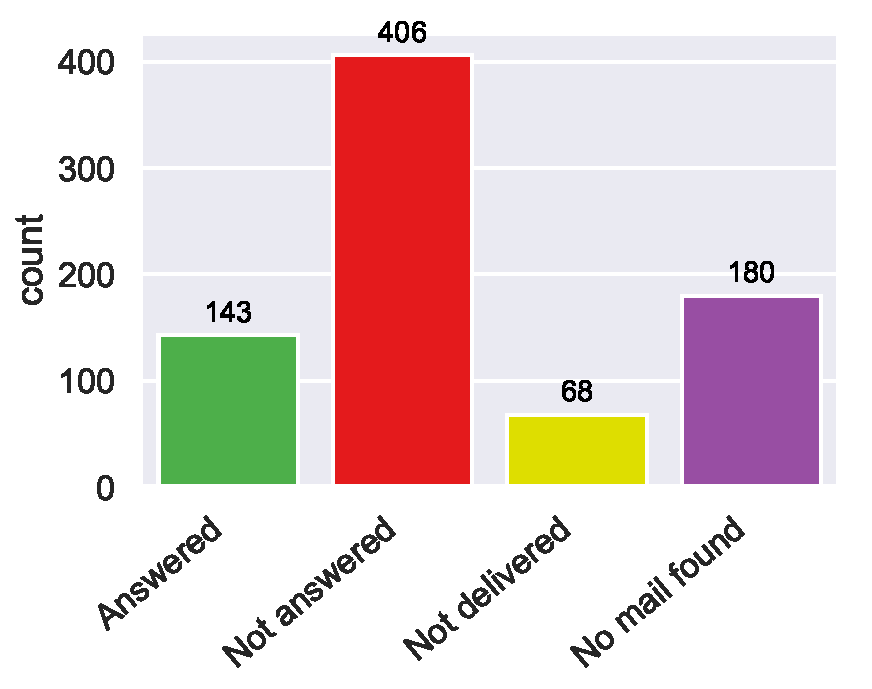
\includegraphics[width=\textwidth, clip]{img/dev-mails/answers-received-builds.pdf}
		\caption{Proportions of logs answered, undelivered and unanswered}
		\label{fig:mails-answers-received-builds}
	\end{minipage}\hfill
	\begin{minipage}{0.45\textwidth}
		\centering
		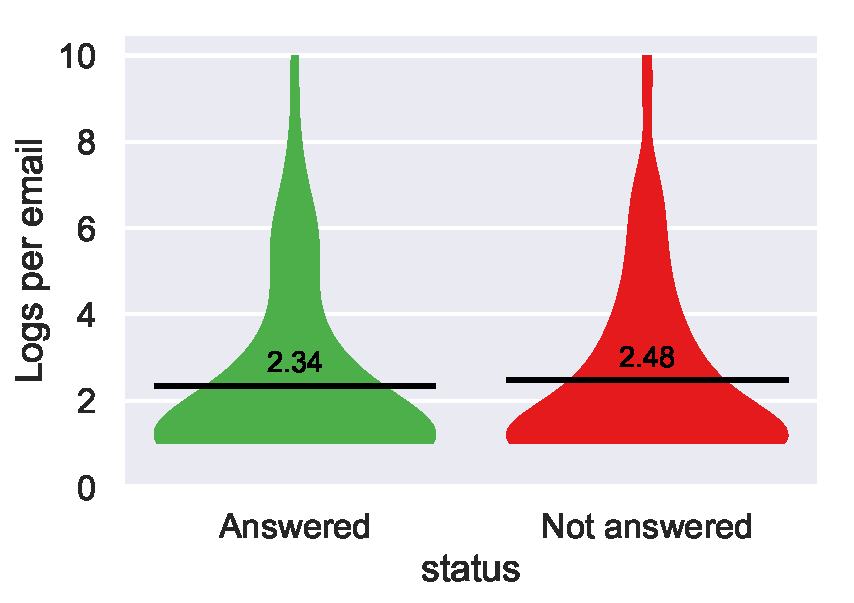
\includegraphics[width=\textwidth, clip]{img/dev-mails/logs-per-mail.pdf}
		\caption{Average number of logs per sent out mail}
		\label{fig:mails-logs-per-mail}
	\end{minipage}
\end{figure}

\subsubsection{Results}
In total we sent out mails to 246 developers, asking about 3.2 build logs on average.
32 of these mails could not be delivered, e.g.\ because they were addressed at noreply mail addresses.
These 32 mails related to 68 of the build logs.
We received answers from 61 developers, responding about 144 build logs.
The proportions of mails and logs answered about, not delivered and unanswered is shown in Figure~\ref{fig:mails-answers-received-mails} and Figure~\ref{fig:mails-answers-received-builds}.

Of the 144 answers, 132 said our extraction was correct.
26 answered either ``close, but not quite correct'' or ``no, the build failed for another reason''.
We manually inspected these negative answers and found that extractions were correct after all.
This yields 12 log extractions in our example set that were not correct, shown in Figure~\ref{fig:mails-extraction-correct}.

\subsubsection{Discussion}
This study highly strengthens the trust in the validity of the extracted build failure reasons in \emph{LogChunks}.
The study received answers about 18\% of the logs labelled in our build log, of which, after manual correction, 91\% said our labelled extractions were accurate.

Most of the initial ``incorrect'' answers we adjusted in them manual inspection, stated that the proposed extraction did not show the whole reason the build failed.
This is because we had to trim long labeled extractions to keep the emails readable.

One of our extractions only showed a warning and the developer propose to also include the line above, stating that warnings are treated as errors in the build.
In others that were identified as ``incorrect'' we labelled the error message of an error that later ignored and did not lead to the build failing.

\subsubsection{Threats to Validity}

\end{document}
